\documentclass[12pt]{article}
\usepackage{graphicx,psfrag,amsfonts,float,mathbbol,xcolor,cleveref}
\usepackage{arydshln}
\usepackage{amsmath}
\usepackage{tikz}
\usepackage[mathscr]{euscript}
\usepackage{subcaption}
\usepackage{mathtools}
\usepackage{IEEEtrantools}
\usepackage{amsthm}
\usepackage[letterpaper, left=1in, top=1in, right=1in, bottom=1in,nohead,includefoot, verbose, ignoremp]{geometry}
\newcommand{\comment}[1]{\text{\phantom{(#1)}} \tag{#1}}
\newcommand\numberthis{\addtocounter{equation}{1}\tag{\theequation}}
\newcommand*\needsparaphrased{\color{red}}
\newcommand*\needscited{\color{orange}}
\newcommand*\needsproof{\color{blue}}
\newcommand*\outlineskeleton{\color{green}}
\newcommand{\PP}{\mathcal{P}}
\newcommand{\bfeps}{\mbox{\boldmath $\epsilon$}}
\newcommand{\bfgamma}{\mbox{\boldmath $\gamma$}}
\newcommand{\bflam}{\mbox{\boldmath $\lambda$}}
\newcommand{\bfphi}{\mbox{\boldmath $\phi$}}
\newcommand{\bfsigma}{\mbox{\boldmath $\sigma$}}
\newcommand{\bfbeta}{\mbox{\boldmath $\beta$}}
\newcommand{\bfalpha}{\mbox{\boldmath $\alpha$}}
\newcommand{\bfe}{\mbox{\boldmath $e$}}
\newcommand{\bff}{\mbox{\boldmath $f$}}
\newcommand{\bfone}{\mbox{\boldmath $1$}}
\newcommand{\bft}{\mbox{\boldmath $t$}}
\newcommand{\bfo}{\mbox{\boldmath $0$}}
\newcommand{\bfO}{\mbox{\boldmath $O$}}
\newcommand{\bfx}{\mbox{\boldmath $x$}}
\newcommand{\bfX}{\mbox{\boldmath $X$}}
\newcommand{\bfz}{\mbox{\boldmath $z$}}


\newcommand{\bfm}{\mbox{\boldmath $m}}
\newcommand{\bfy}{\mbox{\boldmath $y$}}
\newcommand{\bfd}{\mbox{\boldmath $d$}}
\newcommand{\bfc}{\mbox{\boldmath $c$}}
\newcommand{\bfa}{\mbox{\boldmath $a$}}
\newcommand{\bfb}{\mbox{\boldmath $b$}}
\newcommand{\bfY}{\mbox{\boldmath $Y$}}
\newcommand{\bfS}{\mbox{\boldmath $S$}}
\newcommand{\bfZ}{\mbox{\boldmath $Z$}}
\newcommand{\cardT}{\vert \mathcal{T} \vert}
%\newenvironment{theorem}[1][Theorem]{\begin{trivlist}
%\item[\hskip \labelsep {\bfseries #1}]}{\end{trivlist}}
%\newenvironment{corollary}[1][Corollary]{\begin{trivlist}
%\item[\hskip \labelsep {\bfseries #1}]}{\end{trivlist}}
%\newenvironment{proposition}[1][Proposition]{\begin{trivlist}
%\item[\hskip \labelsep {\bfseries #1}]}{\end{trivlist}}
%\newenvironment{definition}[1][Definition]{\begin{trivlist}
%\item[\hskip \labelsep {\bfseries #1}]}{\end{trivlist}}

\newtheorem{theorem}{Theorem}[section]
\newtheorem{lemma}[theorem]{Lemma}
\newtheorem{proposition}[theorem]{Proposition}
\newtheorem{corollary}[theorem]{Corollary}

\theoremstyle{definition}
\newtheorem{definition}{Definition}[section]
\newtheorem{example}{Example}[section]
\def\bL{\mathbf{L}}


\makeatletter
\renewcommand{\theenumi}{\Roman{enumi}}
\renewcommand{\labelenumi}{\theenumi.}
\renewcommand{\theenumii}{\Alph{enumii}}
\renewcommand{\labelenumii}{\theenumii.}
\renewcommand{\p@enumii}{\theenumi.}
\makeatother

 \begin{document}

\nocite{*}


\section{A representation for piecewise polynomial functions}

Let $\xi = \left\{ \xi_1<\xi_2<\dots<\xi_{l+1} \right\}$ be a set of strictly increasing series of points, and let $k$ be a positive integer. Further, let $P_1,\dots,P_l$ denote a sequence of $l$ polynomials of order $k$. Then the correponding piecewise polynomial (pp) function of order $k$ is defined as follows:

\[
f\left(x\right) = P_i\left(x\right) \; \textup{if } \xi_i < x < \xi_{i+1}
\] 
\noindent
for $i=1,\dots,l$. $\left\{\xi\right\}$ are known as the breakpoints of $f$. At the interior breakpoints, $\xi_2,\dots, \xi_l$, the function value is defined by specifying $f$ to be right continuous; that is, 
\[
f\left(\xi_i\right) = f\left(\xi_i^+\right),\quad i=2,\dots,l
\]
However, in a sense, without this specification, the function has two values at any interior breakpoint: the value it gets from the polynomial piece to the left of the breakpoint, $f\left(\xi_i^-\right) = P_{i-1}\left(\xi_i\right)$, in addition to the value it gets from the polynomial piece to the right of the breakpoint, $f\left(\xi_i^+\right) = P_{i}\left(\xi_i\right)$. To properly define the function, one can specify $f$ to be right-continuous:
\begin{equation}
f\left(\xi_i\right) \equiv f\left(\xi_i^+\right) 
\end{equation}

Denote the set of pp functions of order $k$ with breakpoints $\xi=\left\{\xi_1,\dots,\xi_{l+1}\right\}$ by 
\[
\mathcal{P}_{k,\xi}.
\]

$\mathcal{P}_{k,\xi}$ is a linear space having dimension $kl$, as it consists of $l$ polynomials, each having $k$ polynomial coefficients. The $j^{th}$ derivative of a pp $f$,
\[
D^jf
\]
\noindent
is a pp function of order $k-j$ having the same breakpoint sequence and constructed from the same $j^{th}$ derivatives of the polynomial pieces from which $f$ was constructed. This ``definition'' dodges much of the complicated discussion of the derivatives of a pp function at its breakpoints and thus must be treated with considerable care in context of the fundamental theorem of calculus.

\begin{proposition} \label{proposition:continuous_function}
A pp function, $f$ satisfies
\[
f\left(x\right) - f\left(a\right) = \int_a^x \left(Df\right)\left(t\right)dt\quad \textup{for all} \quad x
\]
if and only if $f$ is a continuous function.
\end{proposition}

Consider a piecewise constant function $f$: by the previous definition, its first derivative is identically zero, and is therefore equal to the usual derivative of $f$ if and only if $f$ is constant. The following definition gives the information necessary for a convenient and efficient representation of this class of functions:

\begin{definition}\label{definition:pp_representation}
The \emph{piecewise polynomial (pp) representation} of a function $f \in \PP_{k,\xi}$ consists of 
\begin{enumerate}
\item integers $k$ and $l$, specifying the order and number of polynomial pieces, respectively,
\item a strictly increasing set of breakpoints, $\xi_1,\xi_2,\dots, \xi_{l+1}$,
\item and the set of values of the right derivatives at each of the breakpoints, 
\[
c_{ij} = D^{j}f\left(\xi_i^+\right), \quad j=1,\dots,k;\quad i=1,\dots,l 
\]
\end{enumerate}
\end{definition} 
 
 \section{The truncated power basis and the spaces $\PP_{k,\xi,\nu}$}
This prerequisite information is merely for the ability to responsibly refer to the set of piecewise polynomial functions and have a shorthand way of doing so. These means enable us to introduce two sets of basis functions: first, the truncated power basis, followed by B-spline basis functions. We will see that both are closely related, with the former having some properties which leave them unattractive for function approximation and thus present the construction of B-splines and how to use them to construct a representation of $\mathcal{P}_{k}$. In practice, one typically is given some information about an unknown function, $g$, and the task is to construct a function $f \in \PP_{k, \xi}$ which satisfies conditions that $g$ also satisfies, and in addition, has a certain number of continuous derivatives. These conditions define a subspace of $\PP_{k,\xi}$, $\PP_{k,\xi, \nu}$ for which we will need a corresponding basis.


\subsection{Example: histogram smoothing by parabolic splines}
For illustrative purposes, consider the task of smoothing a histogram using parabolic splines. Suppose we are given points
\[
\tau_1 < \tau_2 < \dots < \tau_{n+1}
\]
and non-negative numbers $h_1, h_2, \dots, h_n$, with $h_i$ denoting the height of the histogram over the interval $\left(\tau_i, \tau_{i+1} \right)$. The histogram is an approximate representation of some underlying density function, $g$. Letting $\Delta \tau_i = \tau_{i+1}-\tau_i$, one may interpret $h_i\Delta \tau_i$ as (approximately) equal to the integral of $g$ over $\left[\tau_i, \tau_{i+1} \right]$. One may impose the following interpolation conditions on our smooth function, $f$:
\begin{equation*} 
\int_{\tau_i}^{\tau_{i+1}} f\left(x\right)dx = h_i\Delta \tau_i
\end{equation*} 
\noindent
for $i=1,\dots, n$. Let $f$ be a piecewise polynomial of order 3 having continuous first derivative:
\[
f \in \PP_{3,\xi} \cap \mathcal{C}^{\left(1\right)}
\]
Choose the breakpoint sequence $\xi$ to coincide with $\tau = \left\{\tau_1,\dots, \tau_{n+1} \right\}$. If $g$ is smooth and vanishes outside its support, $\left[ \tau_1,\tau_{n+1} \right]$, then
\[
g^{\left( j \right)}\left(\tau_1\right) = g^{\left( j \right)}\left(\tau_{n+1}\right) = 0,
\]
\noindent
for $j=0,1,\dots,d$, where $d$ characterizes the extent of the smoothness of $g$, we may also wish to require $f$ to obey two additional interpolation constraints:
\[
f\left( \tau_1 \right) = f\left( \tau_{n+1} \right) = 0,
\]
giving a total of $n+2$ interpolation conditions. These, along with the $2\left(n-1\right)$ continuity conditions yield a total $3n$ constraints on the $3n$ polynomial coefficients,
\[
c_{ji} \equiv D^{j-1} f\left(\xi_i^+ \right).
\]
These conditions lead to the system of equations:

\begin{align*}
c_{11} &  &  &  &  &  &  & & & & & & & &&&&= & 0  \\
c_{11} & \;+\;  & c_{21} \frac{\Delta\tau_{1}}{2!} & \;+\;   & c_{31} \frac{\left(\Delta\tau_{1}\right)^2} {3!}  & 			   & 		 		        &  	      & & & && & &&&& = & h_1\\
c_{11} & \; +\; & c_{21}\Delta\tau_{1}                 & \; + \; & c_{31}\frac{2\left(\Delta\tau_{1}\right)^2}{3!}  & \;-\; & c_{12} &  		        & 	      & & & & & &&&& = & 0\\
\vdots   &  		   & c_{21}  				     & \; + \; & c_{31} \Delta\tau_{1}  				     &  		   &  		 & \;-\;  & c_{22} & && & & &&&& = & 0\\
	   &  			   &             				     &                        & 								     &  		   &   c_{12} &\;+\; &  c_{22}\frac{\Delta\tau_2}{2} &\;+\; & c_{32}\frac{\left(\Delta\tau_2\right)^2}{3!} & & & & &&& = & h_2\\
	   &  			   &             				     &                        & 								     &  		   &   c_{12} &\;+\; &  c_{22}\Delta\tau_2        &\;+\; & c_{32}\frac{\left(\Delta\tau_2\right)^2}{2} & & &\dots &&&&  = & 0\\
	   	   &  			   &             				     &                        & 								     &  		   &   		 &	&  c_{22}        &\;+\; & c_{32}\Delta\tau_2 & & & \dots &&&&  = & 0\\
    &  &  &  &  &  &  & & & & && & &&&&  &\\
   &  &  &  &  &  &  & & & & && & &\ddots &&&  & \numberthis  \label{eq:histogram_smoothing_eqn_system}
\end{align*}

\subsection{The subspace, $\PP_{k,\xi,\nu}$}
One may quickly see that this system is two-thirds homogeneous; that is, for every integral interpolation constraint, we have two continuity constraints that lead to zeros on the right hand side of the equality. To solve \ref{eq:histogram_smoothing_eqn_system}, the homogeneous equations are solved, leaving a reduced set of equations. To do this, one may construct a set of linearly independent functions $\phi_1, \phi_2, \dots$ of the same size as the number of interpolation constraints which satisfy the homogeneous equations in \ref{eq:histogram_smoothing_eqn_system}. The smoother, $f$, is then constructed within this subspace of $\PP_{3,\xi}$ and has form 
\[
f = \sum_{j} \alpha_j \phi_j.
\] 

\noindent
The $\left\{ \phi_j \right\}$ span a particular subspace of $\mathcal{P}_{k, \xi}$, which is comprised of functions which satisfy the homogeneous equations in \ref{eq:histogram_smoothing_eqn_system}. In general, we may characterize these homogeneous equations in terms of a given function having a particular number of continuous derivatives, which may be expressed as follows:
\begin{eqnarray}
\mathscr{J}_{ij}f = 0, \quad  i&=&2,\dots,l \label{eq:tpf_linear_operator_penalty} \\
 j&=&1,\dots,\nu_i \nonumber
\end{eqnarray}
\noindent
where
\begin{equation}
\mathscr{J}_{ij}f = \lim_{x\rightarrow \xi^+} D^{j-1}f\left(x\right) - \lim_{x\rightarrow \xi^-} D^{j-1}f\left(x\right)
\end{equation}
\noindent
and $\nu = \left(\nu_1,\dots, \nu_l\right)$ is a vector of non-negative integers. Each $\nu_i$ specifies the number of continuity conditions impose on the function at the $i^{th}$ breakpoint, $\xi$, and $\mathscr{J}_{ij}$ is simply the size of the jump in the $\left(j-1\right)^{st}$ derivative at $\xi$.


\subsection{The truncated power functions}
As homogeneous conditions specified in \ref{eq:tpf_linear_operator_penalty} are done so in terms of a linear operator applied to the functions in the space, those functions $\left\{ g \in \PP_{k,\xi} \right\}$ constitute a linear subspace, denoted
\[
 \PP_{k,\xi, \nu} 
\]
\noindent
Now that the subspace is defined, we need a basis for it. One such candidate set of basis functions is the truncated power basis. Define

\[
\left(x-t\right)_+ = \max\left(0,x-t\right)
\]
\noindent
We may then define the truncated power function as follows:
\begin{align}
\begin{split}
\left(x-t\right)_+^p &= \left( \left(x-t\right)_+\right)^p\\
&= \left\{\begin{array}{lr}
	\left(x-t\right)^p, & x \ge t\\
	0 & x < t
	\end{array} \right.
	\end{split}
\end{align}

The function $g\left(x\right) = \left(\right)_+^p$ is a piecewise polynomial with a single breakpoint at $\xi$, and is continuous at this breakpoint for $p>0$. For $p=0$, it has a jump of size 1 at $\xi$. Since

\[
D\left( \cdot - \xi\right)_+^p = p \left( \cdot - \xi\right)_+^{p-1},
\]
\noindent
it is clear that $g$ has $p-1$ continuous derivatives. Define the set of linear operators $\left\{ \lambda_{ij} \right\}$ and corresponding functions $\left\{ \phi_{ij} \right\}$ as follows:

\begin{align}
\begin{split}
\lambda_{ij}f  &= \left\{\begin{array}{lr}
	 D^{j}f\left(\xi \right) & i=1\\
	D^{j}f\left(\xi^+ \right) -  D^{j}f\left(\xi^-\right) & i=2,\dots,l
	\end{array} \right. \\
\phi_{ij}\left(x\right) &= \left\{\begin{array}{lr}
	\frac{\left(x-\xi_i \right)^p}{j!} & i=1\\
	\frac{\left(x-\xi_i \right)_+^p}{j!} & i=2,\dots,l
	\end{array} \right. 	
	\end{split} \label{eq:PP_basis_decomposition_componenents}
\end{align}
\noindent for $j=0,\dots,k-1$. Per this definition, we have that $\phi_{ij} \in \PP_{k,\xi}$ for each $i=1,\dots,l$. Further, we have that 

\begin{align*}
\lambda_{ij}\phi_{pq} = \left\{\begin{array}{lr}
	1  & i=p,\;j=q\\
	0 & \textup{otherwise}
	\end{array} \right. ,
\end{align*}
\noindent
making $\left\{ \phi_{ij} \right\}$ a set of $kl$ linearly independent functions, and since $\PP_{k,\xi}$ has dimension $kl$, they constitute a basis for the space. We may represent any $g \in \PP_{k,\xi}$ in the form

\begin{equation*}
g = \sum_{i,j} \left(\lambda_{ij}g\right)\phi_{ij}
\end{equation*}
\noindent
Rewriting this expansion in the terms presented in \ref{eq:PP_basis_decomposition_componenents}, we have that we may express any function in the space as
\begin{equation} \label{eq:tpf_basis_expansion}
g\left(x\right) = \sum_{j=0}^{k-1} \left[ D^j g\left(\xi_1\right)\frac{\left(x-\xi_1\right)^j}{j!} + \sum_{i=2}^l \left[ D^j g\left(\xi_i^+\right)-D^j g\left(\xi_i^-\right) \right]\frac{\left(x-\xi_i\right)_+^j}{j!} \right]
\end{equation}

From this representation of the function, one can see that the coefficients of the basis functions are explicitly defined in terms of jumps of various derivatives of $g$ at the breakpoints. Thus, enforcing the homogeneous constraints 
\[
\mathscr{J}_{ij}f = 0, \quad i=2,\dots, l;\quad j=1,\dots,\nu_i
\]
is accomplished simply by restricting our attention to functions of the form \ref{eq:tpf_basis_expansion} for which these coefficients are zero. This implies that the reduced set of basis functions $\left\{ \phi_{ij} \right\}$, $i=1,\dots,l$, $j=\nu_{i},\dots,k-1$ is a basis for the subspace, $\PP_{k,\xi,\nu}$. (We let $\nu_1 =0$.) Then, every function $g^* \in \PP_{k,\xi}$ in satisfying the homogeneous equations may be written in exactly one way of the form
\begin{equation} \label{eq:tpf_subspace_basis_expansion}
g^* = \sum_{i=1}^l \sum_{j={\nu_i}}^{k-1} \alpha_{ij} \phi_{ij}
\end{equation}

\subsubsection{The pitfalls of the truncated power basis}

While the truncated power basis initially appears quite attractive for smoothing problems involving piecewise polynomials, they exhibit properties that can lead to poor function representations. In order to discuss these characteristics, we must first introduce the notion of the \emph{condition} of a function representation.

\begin{definition}\label{definition:basis_condition}
Consider a piecewise polynomial representation of a function, $p$:
\begin{equation} \label{eq:polynomial_representation}
p = \sum_{i=1}^n a_i P_i
\end{equation}
\noindent
where $a = \left(a_1,\dots,a_n\right)$ is a coefficient vector and $\left\{ P_i\right\}$ is a set of polynomial functions defined on a closed interval $\left[a,b\right]$. We define the \emph{size} of the polynomial $p$ to be
\[
\left \lVert p \right \rVert = \max_{a\le x\le b} \left \lvert p\left(x\right) \right \rvert,
\]
\noindent
and similarly, we define the size of the coefficient vector $a$ to be
\[
\left \lVert a \right \rVert = \max_{1\le i \le n} \left \lvert a_i \right \rvert,
\]
Then, we can bound the size of the function $p$:
\begin{equation} \label{eq:polynomial_expansion_size_bounds}
m\left \lVert a \right \rVert \le \left \lVert \sum_{i=1}^n a_i P_i \right \rVert \le  M \left \lVert a \right \rVert
\end{equation}
\noindent
where 
\begin{align*}
m &= \min_a \frac{\left \lVert \sum_{i=1}^n a_i P_i \right \rVert}{\left \lVert a \right \rVert},\quad \textup{and}\\
M &= \min_a \frac{\left \lVert \sum_{i=1}^n a_i P_i \right \rVert}{\left \lVert a \right \rVert}
\end{align*}
The \emph{condition} of the representation of $p$ as written in \ref{eq:polynomial_representation} is given by 
\[
\textit{condition}\left( P_i \right) = \frac{M}{m}
\]
\end{definition}

The condition of a function representation quantifies the extent to which a slight change in the coefficient vector will impact the function itself. To see this, rather than the coefficient vector $a$, consider instead a perturbation of $a$:
\[
a + \delta a
\]
\noindent
The corresponding perturbed polynomial is given by 
\[
p + \delta p = \sum_{i=1}^n \left(a_i + \delta a_i \right) P_i
\]
By \ref{eq:polynomial_expansion_size_bounds}, we then have that 
\begin{equation*}
\frac{m\left \lVert \delta a \right \rVert}{M\left \lVert a \right \rVert} \le \frac{\left \lVert \delta p \right \rVert}{\left \lVert p \right \rVert} \le \frac{M\left \lVert \delta a \right \rVert}{m\left \lVert a \right \rVert},
\end{equation*}
\noindent
implying that a relative change of $\frac{\left \lVert \delta a \right \rVert}{\left \lVert a \right \rVert}$ to the coefficient vector may result in a relative change to the function $p$ as large as $\frac{M}{m} = \textit{condition}\left(P_i\right)$ times the relative change in $a$ (and at least as large as $\textit{condition}\left(P_i\right)^{-1}$). Note that the width of the interval 
\[
\left[\textit{condition}\left(P_i\right)^{-1}\frac{\left \lVert \delta a \right \rVert}{\left \lVert a \right \rVert},\textit{condition}\left(P_i\right) \frac{\left \lVert \delta a \right \rVert}{\left \lVert a \right \rVert} \right]
\]
\noindent
is increasing in $\textit{condition}\left(P_i\right)$; so large values of the condition of a representation imply that small relative changes in their corresponding coefficients may result in much smaller or much larger relative changes in the function being represented.

When representing a function $f \in \PP_{k,\xi}$ as in \ref{eq:tpf_basis_expansion}, two issues of concern arise: first, if $l$ is large, the value of the function at a point $x$ can potentially rely on far more than just $k$ of the basis coefficients. Additionally, if the breakpoints $\xi$ are very irregularly spaced, then the truncated power basis can present poor condition, which, in turn, can result in poorly conditioned linear systems (like the specific example given by \ref{eq:histogram_smoothing_eqn_system}.) Consequently, small perturbations of the basis function coefficients result in disproportional changes in the function.
\begin{figure}[H] 
\begin{center}
\begin{tikzpicture}
\draw[->] (-1,0) -- (11,0);
\draw[->] (0,-1) -- (0,3.5);
\filldraw[black] (0.1,1.3) circle (2pt)  ;
\filldraw[black] (1.1,1.3) circle (2pt)  ;
\filldraw[black] (2.1,1.3) circle (2pt)  ;
\filldraw[black] (3.1,1.3) circle (2pt)  ;
\filldraw[black] (4.45,2.4) circle (2pt)  ;
\filldraw[black] (4.75,0.2) circle (2pt)  ;
\filldraw[black] (6.1,1.3) circle (2pt)  ;
\filldraw[black] (7.1,1.3) circle (2pt)  ;
\filldraw[black] (8.,1.3) circle (2pt)  ;
\filldraw[black] (9.1,1.3) circle (2pt)  ;
\filldraw[black] (10,1.3) circle (2pt)  ;

\draw (0.1,1.3) -- (3.1,1.3);
\draw (3.1,1.3) -- (4.45,2.4);
\draw (4.45,2.4) -- (4.75,0.2);
\draw (4.75,0.2) -- (6.1,1.3);
\draw (6.1,1.3) -- (10,1.3);
\draw (0.1,0) node[above,scale=0.6] {$\xi_{1}$};
\draw (1.1,0) node[above,scale=0.6] {$\xi_{2}$};
\draw (2.1,0) node[above,scale=0.6] {$\xi_{3}$};
\draw (3.1,0) node[above,scale=0.6] {$\xi_{4}$};

 \draw (4.45,-.38) -- (4.45,-.22); 
 \draw (4.75,-.38) -- (4.75,-.22); 
\draw (4.45,-.3) -- (4.75,-.3) ;
\draw (4.6,-0.3) node[below,scale=0.6,align=center] {h};

\draw (6.1,0) node[above,scale=0.6] {$\xi_{7}$};
\draw (7.1,0) node[above,scale=0.6] {$\xi_{8}$};
\draw (8.1,0) node[above,scale=0.6] {$\xi_{9}$};
\draw (9.1,0) node[above,scale=0.6] {$\xi_{10}$};
\draw (10,0) node[above,scale=0.6] {$\xi_{11}$};
\foreach \coo in {.1,1.1,...,3.1}
{
  \draw (\coo,-1.5pt) -- (\coo,1.5pt); 
  \draw (\coo,0) node[below,scale=0.6] {\coo};
}
 \draw (4.45,-1.5pt) -- (4.45,1.5pt);
  \draw (4.75,-1.5pt) -- (4.75,1.5pt);
\foreach \coo in {6.1,7.1,...,9.1}
{
  \draw (\coo,-1.5pt) -- (\coo,1.5pt);
  \draw (\coo,0) node[below,scale=0.65] {\coo};
}
 \draw (10,0) node[below,scale=0.65] {10};
\draw (10,-1.5pt) -- (10,1.5pt);
\draw (-1.5pt,0.2) -- (1.5pt,0.2);
\draw (-1.5pt,1.3) -- (1.5pt,1.3);
\draw (-1.5pt,2.4) -- (1.5pt,2.4);
\draw (0,0.2) node[left,scale=0.6] {0.2};
\draw (0,1.3) node[left,scale=0.6] {1.3};
\draw (0,2.4) node[left,scale=0.6] {2.4};
\end{tikzpicture} 
\caption{The linear system for the coefficients of the truncated power basis is ill-conditioned for the above piecewise linear function  and choice of breakpoints, $\xi_1,\dots, \xi_{11}$.} \label{fig:piecewise_linear_tpf_fail}
\end{center}
\end{figure}


\begin{example} \label{ex:tpf_fail}
Suppose we wish to construct a function $f \in \PP_{k=2,\xi} \cap \mathscr{C}^{\left(0\right)}$ satisfying $f\left(\xi_i \right)=1.3$ for $i=1,\dots,4,7,\dots,11$, $f\left(\xi_5\right)=2.4$, and $f\left(\xi_6\right)=0.2$ with breakpoints specified as pictured in Fig~\ref{fig:piecewise_linear_tpf_fail}. 


The function $f$ is piecewise linear, so that $f \in \PP_{2,\xi,\nu}$ with $\nu_i=1$, $i=1,\dots, 11$. Then, for $f$ is of the form
\[
f\left(x\right) = \alpha + \beta\left(x-\xi_1\right) + \sum_{i=2}^l\alpha_i\left(x-\xi_i\right)_+
\]
\noindent

one can show that, given the continuity and interpolation constraints, $\alpha = 1.3$, $\beta = f^\prime\left(\xi_1\right) = 0$,  $\alpha_i = 0$ for $i \not \in \left\{4,5,6,7\right\}$, and 
\[
\begin{bmatrix}
\alpha_4\\
\alpha_5\\
\alpha_6\\
\alpha_7\\
\end{bmatrix} =  \begin{bmatrix}
\frac{1.1}{\Delta\xi_4}\\
-\frac{2.2}{\Delta \xi_5} -\frac{1.1}{\Delta\xi_4}\\
\frac{1.1}{\Delta\xi_6} + \frac{2.2}{\Delta \xi_5}\\
-\frac{1.1}{\Delta\xi_6} 
\end{bmatrix} = \begin{bmatrix}
\frac{1.1}{\Delta\xi_4}\\
-\frac{2.2}{h} -\frac{1.1}{\Delta\xi_4}\\
\frac{1.1}{\Delta\xi_6} + \frac{2.2}{h}\\
-\frac{1.1}{\Delta\xi_6} 
\end{bmatrix}
\]

When $h = \Delta \xi_5 \rightarrow 0$, we have 
\begin{align*}
\left(x-\xi_5\right)_+ &\approx \left(x-\xi_6\right)_+\\
\alpha_5  &\approx -\alpha_6 >> 1,
\end{align*}
\noindent
leading to a loss of significance in the evaluation of the function. For example, if we were to choose $\xi_5=4.5$, $\xi_6=4.8$, making $h=0.3$, with five significant decimal digit arithmetic, then we get
\[
\alpha=1.30000,\; \beta= 0.00000,\;\alpha_4= 0.78571,\;\alpha_5= -8.11905,\;\alpha_6= 8.17949,\;\alpha_7= -0.84615
\]
and the other $\alpha_i=0$. Evaluating the corresponding function at $x=9.6$ yields $1.299987$ rather than the correct value of 1.3. This error becomes larger as $h$ approaches 0.
\end{example}

A quick remedy for the problem in \ref{ex:tpf_fail} is to replace the truncated power basis with the set of hat functions:

\[
H_i\left(x\right)=\left\{
\begin{array}{lr}
\left(x-\xi_i\right)/\Delta\xi_{i-1}, & \xi_{i-1} < x \le \xi_i\\
\left(\xi_{i+1}-x\right)/\Delta\xi_{i}, & \xi_{i} < x \le \xi_{i+1}\\
0 & otherwise
\end{array}  \right.
\]
\noindent
To utilize the hat functions, we augment $\xi_1,\dots,\xi_12$ with two additional breakpoints: $\xi_0 \le \xi_1$ and $\xi_{12} \ge \xi_{11}$. Then,

\begin{align*}
f\left(x\right) = 1.3H_1\left(x\right) + \dots + 1.3H_4\left(x\right) &+ 2.4H_5\left(x\right) \\
 &+   0.2H_6\left(x\right)+ 1.3H_7\left(x\right) + \dots + 1.3H_{11}\left(x\right)
\end{align*}

Even just using just two decimal digit arithmetic, we have $f\left(9.5\right) = 1.3$. Even as $h \rightarrow 0$, $f$ is well represented using the hat functions as a basis. More generally speaking, \emph{B-splines}, which are a generalization of these hat functions, overcome the issues that accompany the truncated power basis previously illustrated. The alternative basis is constructed by assembling linear combinations of the truncated power functions, forming a set of basis functions having ``small'' support: the functions vanish outside a small interval of their domain. In the following section, we will define the $k^{th}$-order B-splines as scaled \emph{divided differences} of truncated power functions. We will also show that every subspace $\PP_{k,\xi,\nu}$ has a basis consisting of these functions, bringing forth a B-spline representation of any pp function. 

\section{The B-spline representation of piecewise polynomial functions}

We will present an introduction to B-splines and their properties in the section to follow. As these basis functions are defined in terms of divided differences of the truncated power functions discussed in the previous section, we must first review the definition and properties of the divided difference operator. While there are many ways of defining divided differences, the following (somewhat nonconstructive definition) is intuitive and adequate for our purposes here.

\subsection{The divided difference}

\begin{definition}\label{definition:divided_difference}
The \emph{$k^{th}$ divided difference} of a function $g$ at the points $\tau_i,\dots,\tau_{i+k}$, denoted
\[
\left[ \tau_i,\dots,\tau_{i+k} \right]g,
\]
is the leading coefficient of the polynomial of order $k+1$ which \emph{agrees with $g$} at $\tau_i,\dots,\tau_{i+k}$.
\end{definition}
This leads us to the following definition:

\begin{definition}\label{definition:agrees_with_g}
Let $\left\{\tau_i \right\}_{i=1}^n$ denote a sequence of points. We say that a function $f$ \emph{agrees with} a function $g$ at $\tau$ if, for every point $\tau$ which occurs $m$ times in $\left\{\tau_i \right\}$, $f$ and $g$ agree up to $m$ derivatives at $\tau$; i.e.
\[
f^{\left(i-1\right)}\left(\tau\right) = g^{\left(i-1\right)}\left(\tau\right), \quad i=1,\dots,m
\]
\end{definition}

\subsubsection{Properties of the divided difference}
Definition~\ref{definition:divided_difference} yields the following properties of the $k^{th}$ divided difference:

\begin{enumerate} \label{dd_properties}
\item \label{eq:dd_property_1} Let $\left\{ p_i \right\}$, $i=1,2,\dots$ denote a sequence of polynomials with $p_i$ having order $i$. If $p_i$ agrees with a function $g$ at $\tau_1,\dots, \tau_i$ for $i=k,k+1$, then 
	\begin{equation*} 
	p_{k+1}\left(x\right) = p_k\left(x\right) + \left(x-\tau_1\right)\cdot \dots \cdot \left(x-\tau_k\right)\left[\tau_1,\dots,\tau_{k+1}\right]g
	\end{equation*}
	\begin{proof}
	Note that $p_{k+1}\left(x\right) - p_{k}\left(x\right)$ is a polynomial of order $k+1$ and vanishes at $\tau_1,\dots,\tau_k$, and, by definition, has $\left[\tau_1,\dots,\tau_{k+1}\right]g$ as its leading coefficient. Consequently, $p_{k+1}-p_k$ is of the form
	\begin{equation*}
	p_{k+1}\left(x\right) - p_{k}\left(x\right) = c\prod_{j=1}^k \left(x-\tau_j\right)
	\end{equation*}
	\noindent
	where 
	\[
	c = \left[\tau_1,\dots,\tau_{k+1}\right]g
	\]
	\end{proof}
	This tells the reader that interpolating polynomials may be constructed using divided differences by adding the interpolation points one by one, giving the \emph{Newton form} of the $n^{th}$ order polynomial which agrees with $g$ at $\tau_1,\dots,\tau_n$:
	\[
	p_n\left(x\right) = \sum_{i=1}^n \left(x-\tau_{1}\right)\times \dots \times \left(x-\tau_{i-1}\right) \left[\tau_1,\dots,\tau_{i-1} \right]g
	\]
\item \label{eq:dd_property_2} $\left[\tau_i,\dots,\tau_{i+k} \right]g$	is symmetric in its arguments $\tau_i,\dots, \tau_{i+k}$ (since the interpolating polynomial depends only on the points of interpolation and not the order in which they are specified.)
\item \label{eq:dd_property_3} $\left[\tau_i,\dots,\tau_{i+k} \right]g$ is a linear operator; if we let 
\[
f= \alpha g + \beta h
\]
\noindent
for some functions $g,h$ and scalars $\alpha, \beta$, then
\[
\left[\tau_i,\dots,\tau_{i+k} \right]f = \alpha\left[\tau_i,\dots,\tau_{i+k} \right]g + \beta\left[\tau_i,\dots,\tau_{i+k} \right]h
\]
\item \label{eq:dd_property_4} If $f=gh$, then
\[
\left[\tau_i,\dots,\tau_{i+k} \right]f  = \sum_{j=i}^{i+k} \left[\tau_i,\dots,\tau_{i+k} \right]g \left[\tau_i,\dots,\tau_{i+k} \right]h 
\]
\item \label{eq:dd_property_5} If $g$ is a polynomial of degree $\le k$, then $\left[\tau_i,\dot,\tau_{i+k}\right]g$ is constant as a function of $\tau_i,\dot,\tau_{i+k}$. In particular,
\[
\left[\tau_i,\dot,\tau_{i+k}\right]g = 0 \quad \forall g \in \PP_{k}
\]
The polynomial which agrees with $g$ at $\tau_i,\dots, \tau_{i+k}$ or any other $k+1$ points must be $g$ itself due to the uniqueness of interpolating polynomials. For more details, we refer the reader to {\needscited{A Practical Guide to Splines, DeBoor}}.
\item \label{eq:dd_property_6} $\left[\tau_i,\dots,\tau_{i+k} \right]g$ is a continuous function of its $k+1$ arguments in case $g\in \mathscr{C}^{\left(k\right)}$ (that is, if $g$ has $k$ continuous derivatives.)
\item \label{eq:dd_property_7} If $g\in \mathscr{C}^{\left(k\right)}$, then there exists a point $\xi$ in the smallest interval containing $\tau_i,\dots,\tau_{i+k}$ such that 
\[
\left[\tau_i,\dots,\tau_{i+k} \right]g = \frac{g^{\left(k\right)}\left(\xi\right)}{k!}
\] 
\item \label{eq:dd_property_8}\[
\left[\tau_i,\dots,\tau_{i+k} \right]g = \left\{\begin{array}{ll}
\frac{g^{\left(k\right)}\left(\tau_i\right)}{k!} & \tau_i= \dots = \tau_{i+k},\;\;g\in \mathscr{C}^{\left(k\right)} \\
\frac{\left[\tau_i,\dots,\tau_{r-1},\tau_{r+1},\dots,\tau_{i+k} \right]g-\left[\tau_i,\dots,\tau_{s-1},\tau_{s+1},\dots,\tau_{i+k} \right]g}{\tau_s-\tau_r} &  \tau_r,\tau_s \textup{ are any two distinct}\\
& \textup{  points in } \left\{\tau_i,\dots,\tau_{i+k}\right\}
\end{array} \right.
\]
\item \label{eq:dd_property_9} Let $\tau = \left\{\tau_i \right\}$, $i=1,\dots,n$ be a nondecreasing sequence, and let $g$ be a ``smooth enough'' function. Define the restriction of $g$ to the sequence $\tau$ to be the vector $g \vert_\tau = \left(g_1,\dots,g_n\right)^T$, where
\[
g_i = g^{\left(r\right)}\left(\tau_i\right),\quad r=\max\left\{j:\;\tau_{i-j}=\tau_i\right\}
\]
For any $1 \le r \le s \le n$, there exist constants $\left\{d_i \right\}$, $i=1,\dots,n$ which depend only on $r$, $s$, and $\tau$ and are free of $g$ such that 
\begin{equation} \label{eq:dd_property_9_punchline}
\left[\right]g = \sum_i=1^n d_i g_i
\end{equation}
\begin{proof}
The proof is done by induction on $s-r$. The statement is obvious for the case where $s-r=0$; all $d_i = 0$ except the constant corresponding to $g\left(\tau_r\right)$, which is equal to $1$. For any $r < s$, if $\tau_r= \dots = \tau_s$, then 
\[
\left[\tau_r,\dots, \tau_s\right]g = \frac{g^{\left(s-r\right)}\left(\tau_r\right)}{\left(s-r\right)!}
\]
so that \ref{eq:dd_property_9_punchline} holds with a single $d_j = \frac{1}{\left(s-r\right)!}$ and all other $d_i = 0$. The index $j \le s$ of the nonzero constant depends only on the number of $\tau_j$ with $j<r$ and $\tau_j = \tau_r$.

Assume that \ref{eq:dd_property_9_punchline} holds for $s-r < k$. Consider $s-r = k$ with $\tau_r < \tau_s$. By the induction hypothesis, there are coefficients $\left\{d_i^\prime\right \}$ and $\left\{d_i^{\prime\prime}\right\}$
\end{proof}
\end{enumerate}

In the following section, we will present B-splines as divided differences of the truncated power basis and present some of their properties which come as a result of the properties of the divided difference presented in this section.

\section{A B-spline representation for pp functions}

\begin{definition} \label{definition:order_k_Bspline}
Let $t= \left\{ t_i \right\}$ denote a non-decreasing sequence. The $i^{th}$ B-spline of order $k$ which corresponds to the knot sequence $t$ is defined by 
\begin{equation} \label{eq:bspline_definition}
B_{i,k,t}\left(x\right) = \left(t_{i+k}-t_i\right)\left[t_i,\dots,t_{i+k}\right]\left(\cdot -x\right)_+^{k-1}
\end{equation}
\end{definition}

The placeholder notation, $\left(\cdot - x\right)_+^{k-1}$, is used to indicate that the $k^{th}$ divided difference of the function $g\left(t \right) = \left(t-x\right)^{k-1}_+$ is obtained by fixing $x$ and applying the divided difference to $g\left(t \right)$ as a function of $t$ alone. Henceforth, we will write $B_i$ rather than $B_{i,k,t}$ when the spline order and knot sequence can be inferred from surrounding context.

\subsection{Properties of B-splines}

\begin{enumerate} \label{eq:BS_properties}
\item \label{eq:BS_property_1} $B_i\left(x\right)$ has isolated support:
\[
B_i\left(x\right) = 0, \quad x \not \in \left[t_{i},t_{i+k}\right]
\]
To see this, note that if $x \not \in \left[t_{i},t_{i+k}\right]$, then $g\left(t \right) = \left(t-x\right)^{k-1}_+$ is a polynomial of degree $< k$ on $\left[t_{i},t_{i+k}\right]$, thus by \ref{dd_properties} \ref{eq:dd_property_5},
\[
\left[t_{i},\dots,t_{i+k}\right]g = 0.
\]
As a result, for a set of B-splines of order $k$ corresponding to the knot sequence $t$, only $k$ of them are nonzero on $\left[t_{j},t_{j+k}\right]$: $B_{j-k+1},B_{j-k+2},\dots,B_{j}$.
\item \label{eq:BS_property_2} The $i^{th}$ B-spline of order is defined as the $k^{th}$ divided difference of $\left(\cdot - x\right)_+^{k-1}$ times a normalization factor: $\left(t_{i+k}-t_i\right)$. This normalization, using \ref{dd_properties} \ref{eq:dd_property_8}, allows us to write 
\[
B_i\left(x\right)=\left[t_{i+1},\dots,t_{i+k} \right]\left(\cdot - x\right)_+^{k-1} - \left[t_{i},\dots,t_{i+k-1} \right]\left(\cdot - x\right)_+^{k-1}
\]
For $x \in \left(t_{j},t_{j+1}\right)$, by \ref{dd_properties} \ref{eq:dd_property_1},
\begin{align}
\sum_{i} B_i\left(x\right) &=  \sum_{i=j+1-k}^{j} B_i\left(x\right) \nonumber\\
&= \sum_{i=j+1-k}^{j} \left[t_{i+1},\dots,t_{i+k} \right] \left(\cdot - x\right)_+^{k-1} - \sum_{i=j+1-k}^{j} \left[t_{i},\dots,t_{i+k-1} \right] \left(\cdot - x\right)_+^{k-1} \nonumber \\
&= \left[t_{j+1},\dots,t_{j+k} \right] \left(\cdot - x\right)_+^{k-1} - \left[t_{j+1-k},\dots,t_{j} \right] \left(\cdot - x\right)_+^{k-1} \nonumber \\
&= 1 - 0 \label{eq:unity_equality}
\end{align}
The last equality in \ref{eq:unity_equality} is a consequence of the following: for $x \in \left(t_j,t_{j+1}\right)$, $g\left(t\right)=\left(t - x\right)_+^{k-1}$ is a $k-1$ degree polynomial with unit leading coefficient on $\left[ t_{j+1},t_{j+k} \right]$, so by \ref{dd_properties} \ref{eq:dd_property_5}, 
\[
\left[ t_{j+1},\dots,t_{j+k} \right]g=1.
\]
On $\left[ t_{j+1-k},t_{j} \right]$, $g$ is identically $0$, hence $\left[ t_{j+1-k},\dots,t_{j} \right]g = 0$.   
\item \label{eq:BS_property_3}Each $B_i\left(x\right)$ is positive on its support. Applying Leibnitz's formula (\ref{dd_properties} \ref{eq:dd_property_4}) to the product
\[
\left[t_i,\dots,t_{i+k} \right]\left(t-x\right)_+^{k-1} = \left[t_i,\dots,t_{i+k} \right]\left(t-x\right) \left(t-x\right)_+^{k-2},
\] 
we have
\begin{align}
\left[t_i,\dots,t_{i+k} \right]\left(t-x\right)_+^{k-1} &=  \left[t_i,\dots,t_{i+k} \right]\left(t-x\right) \left(t-x\right)_+^{k-2} \nonumber\\
&= \sum_{r=i}^{i+k}\left[t_i,\dots,t_{i+r} \right] \left(t-x\right)\left[ t_r,\dots,t_{i+k}\right]\left(t-x\right)_+^{k-2} \nonumber \\
&= \bigg[ \left[t_i\right]\left(t-x \right) \bigg]\bigg[ \left[ t_i,\dots,t_{i+k}\right]\left(t-x\right)_+^{k-2}\ \bigg]\nonumber \\
& \qquad \qquad + \bigg[ \left[t_i,t_{i+1}\right]\left(t-x \right) \bigg]\bigg[ \left[ t_{i+1},\dots,t_{i+k}\right]\left(t-x\right)_+^{k-2} \bigg] \nonumber \\
&= \left(t_i-x \right) \left[ t_{i},\dots,t_{i+k}\right]\left(t-x\right)_+^{k-2} \nonumber \\
& \qquad \qquad \qquad \qquad \qquad +  1 \cdot \left[ t_{i+1},\dots,t_{i+k}\right]\left(t-x\right)_+^{k-2} \label{eq:nonneg_star}
\end{align}
since $\left[ t_i,\dots,t_j\right]\left(\cdot-x\right) = 0$ for $j>i+1$. By \ref{dd_properties} \ref{eq:dd_property_8}, 
\[
\left(t_i-x \right) \left[ t_{i},\dots,t_{i+k}\right]g = \frac{t_i-x}{t_{i+k}-t_{i}}\bigg[\left[ t_{i+1},\dots,t_{i+k}\right]g -\left[ t_{i},\dots,t_{i+k-1}\right]g   \bigg],
\]
and we may express \ref{eq:nonneg_star} as 
\begin{align*}
\left[ t_{i},\dots,t_{i+k}\right]\left(\cdot - x\right)^{k-1}_+ &= \frac{x-t_i}{t_{i+k}-t_{i}}\left[ t_{i},\dots,t_{i+k-1}\right] \left(\cdot-x\right)_+^{k-2}  \\
& \quad + \frac{t_{i+k}-x}{t_{i+k}-t_{i}}\left[ t_{i+1},\dots,t_{i+k}\right] \left(\cdot-x\right)_+^{k-2} 
\end{align*}
which we can write in terms of the normalized B-spline:
\begin{equation} \label{eq:nonneg_starstar}
\frac{B_{i,k}\left(x\right)}{t_{i+k}-t_i} = \frac{x-t_i}{t_{i+k}-t_{i}}\frac{B_{i,k-1}\left(x\right)}{t_{i+k-1}-t_i} + \frac{t_{i+k}-x}{t_{i+k}-t_{i}} \frac{B_{i+1,k-1}\left(x\right)}{t_{i+k}-t_{i+1}}
\end{equation}
This shows that we can write the $i^{th}$ B-spline of order $k$ as a convex combination of the $i^{th}$ and $\left(i+1\right)^{st}$ B-splines of order $k-1$ since 
\[
\frac{x-t_i}{t_{i+k}-t_{i}} + \frac{t_{i+k}-x}{t_{i+k}-t_{i}}  = 1,
\]
and each of these weights are positive for $t_i < x < t_{i+1}$. If
\[
\begin{array}{lr}
B_{j,k-1}\left(x\right) > 0, & t_j < x < t_{j+k-1} \; \textup{for all } j,
\end{array}
\]
then by \ref{eq:nonneg_starstar}, we have that 
\[
B_{i,k}\left(x\right) > 0,  \qquad t_i < x < t_{i+k}
\]
since $B_{j,k-1}= 0$ for $x \not \in \left[t_j,t_{j+k}\right]$ by \ref{eq:BS_properties} \ref{eq:BS_property_1} and by induction over $k$, starting with the fact that 
\[
B_j,1\left(x\right) = \left\{ \begin{array}{lr}
1 & t_j \le x < t_{j+1}\\
0 & otherwise
\end{array}\right.
\]
Properties \ref{eq:BS_property_1}, \ref{eq:BS_property_2}, and \ref{eq:BS_property_3} demonstrate that a sequence of B-splines form a \emph{partition of unity}: a set of non-negative functions which sum, pointwise, to one.
\end{enumerate}

\begin{example}
Figure~\ref{fig:deboor_bspline_basis} show fives parabolic B-splines corresponding to the set of knots $\left\{0,1,1,3,4,6,6,6 \right\}$. It is clear that each spline has compact support and is non-negative on this support. The function values are provided at select domain values so that property \ref{eq:BS_property_2} is evident, though it is worth noting that 
\[
\sum_{i=1}^6 B_i\left(x\right) = 1
\]
only on $\left[\frac{1}{6},1\right]$. In particular, they do not sum to 1 on $\left(0,\frac{1}{6}\right)$. 

Each $B_i$ is piecewise parabolic, with the breakpoints being locations of discontinuity of the function or one of its derivatives. $B_5$ is discontinuous at $x=6$, as the knot at 6 is repeated three times in the knot sequence defining $B_5$: $\left\{t_5,t_6,t_7,t_8\right\}$.

$B_1$, $B_2$, and $B_4$ have discontinuous first derivatives since 1 is repeated twice in the knots defining $B_1$ and $B_2$, and 6 is repeated twice in the knots defining $B_4$. The relationship between knot replication and smoothness will be discussed in more detail in the following section.

\begin{figure}[h]
 \begin{center}
 \graphicspath{{img/}}
  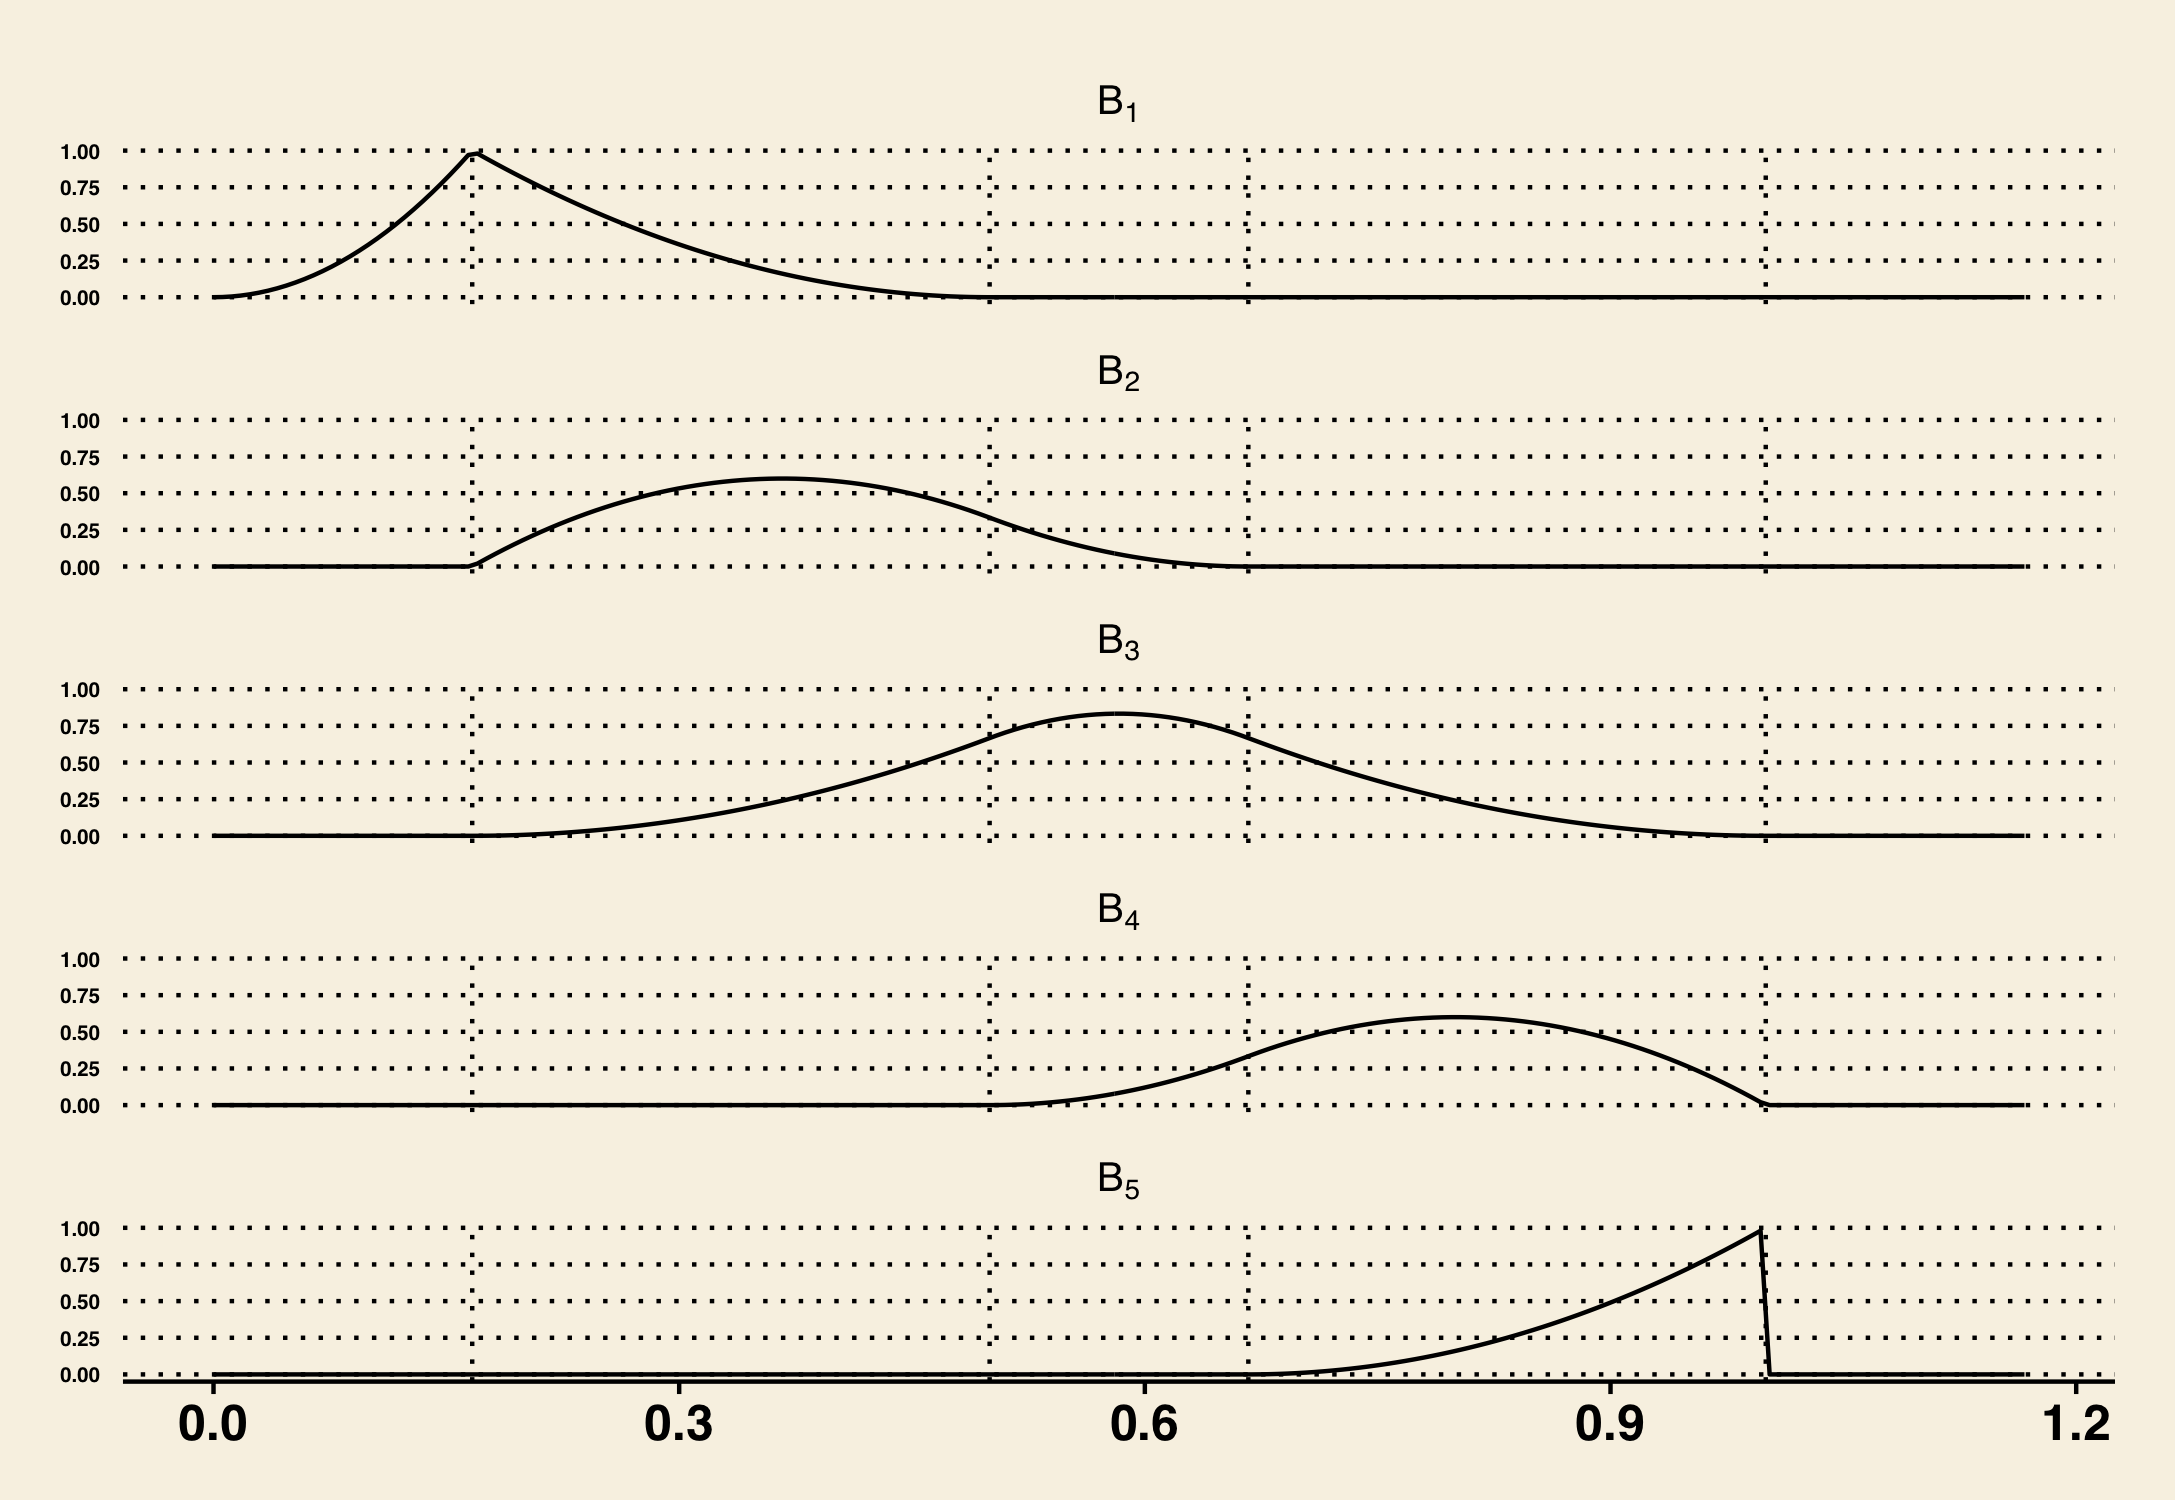
\includegraphics[width=7in, height=5in]{deboor_parabolic_bsplines.png}
  \caption{Parabolic B-splines corresponding to knot sequence $\{0,1,1,3,4,6,6,6\}$, illustrating the connection between knot multiplicity and smoothness.}\label{fig:deboor_bspline_basis}
\end{center}
\end{figure}
\end{example}

\subsection{The Curry-Schoenberg Theorem}

There is an extensive body of literature 
\begin{definition}
A \emph{spline function of order k with knot sequence t} is any linear combination of B-splines of order $k$ for the knot sequence $t$. We denote this set of functions by 
\[
\mathscr{S}_{k,t} = \bigg\{ \sum_i \alpha_i B_{i,k,t}: \quad \alpha_i \in \Re \bigg \}
\]
\end{definition}

\begin{theorem}{Curry-Schoenberg Theorem} \label{curryschoenbergthm}
For a strictly increasing sequence $\xi = \big\{ \xi_i \big\}$, $i=1,\dots, l+1$ and a sequence of non-negative integers $\nu = \big\{ \nu_j \big\}$, $j=2, \dots,l$ with $\nu_j \le k$ for all $j$, define
\begin{align*}
n &= k + \sum_{i=2}^l\left(k-\nu_i\right) = kl - \sum_{i=2}^l \nu_i \\
&= \textup{dim}\left(\PP_{k,\xi,\nu}\right)
\end{align*}
and let 
$t = \big\{ t_i \big\}$, $i=1, \dots,n+k$ be a non-decreasing sequence with 
\begin{enumerate}
\item \begin{align*}
 t_1 & \le t_2 \le  \dots \le t_{k} \le \xi_1\\
 \xi_{l+1} & \le t_{n+1} \le  \dots \le t_{n+k}\\
\end{align*}
\item $\xi_i$ occurs exactly $k-\nu_i$ times in $t$ for $i=2,\dots,l$.
\end{enumerate}
Then, the sequence of B-splines of order $k$ for the knot sequence $t$, $B_1,\dots, B_n$, is a basis for $\PP_{k,\xi,\nu}$ on the domain $\left[t_k,t_{n+1} \right]$. 
\end{theorem}

Theorem~\ref{curryschoenbergthm} gives an explicit prescription for the construction of a B-spline basis for any particular pp space, $\PP_{k,\xi,\nu}$, via the specification of $t$. These functions were named (B for `basis') for this theorem. The choice of $t$ controls the smoothness of the corresponding basis functions via knot multiplicities; the number of knots at a given breakpoint dictates the amount of smoothness at the breakpoint. Fewer knots placed at a breakpoint leads to more continuity conditions such that 
\[
\left[\mbox{\# continuity conditions at } \xi\right] + \left[\mbox{\# knots at } \xi\right] = k
\]
A knot with multiplicity $k$ yields a basis with no continuity conditions at that point, and a point where there are no knots forces $k$ continuity conditions there.

\subsubsection{The Curry-Schoenberg Proof}

\begin{proof}
We begin by showing that $B_i \in \PP_{k,\xi,\nu}$ for all $i$ as functions defined on $\left[t_k,t_{n+1}\right]$. Each $B_i = B_{i,k,t}$ is defined as the $k^{th}$ divided difference of $\left(t-x\right)_+^{k-1}$ at $t_i,\dots,t_{i+k}$ times a scalar, so by \ref{dd_properties} \ref{eq:dd_property_9}, we can find coefficients $d_i,\dots,d_{i+k}$ which depend only on $t_{i},\dots,t_{i+k}$ so that for any smooth function $g$, 
\begin{equation} \label{eq:cs_proof_star}
\left[t_i,\dots,t_{i+k} \right]g = \sum_{r=i}^{i+k} d_r g^{\left(j_r\right)}\left(t_r\right)
\end{equation}
with 
\[
j_r = \max \bigg\{s:\;\;r-s \ge i \mbox{ and } t_{r-s} = t_r;\;\;r=i,\dots,i+k\bigg\}.
\]
Using this, we may write 
\begin{equation} \label{eq:cs_proof_starstar}
B_i\left(x\right) = \left(t_{i+k}-t_i\right)\sum_{r=i}^{i+k} d_r \left(t_r - x\right)_+^{k-j_r-1}\frac{\left(k-1\right)!}{\left(k-j_r-1\right)!}.
\end{equation}
From \ref{eq:cs_proof_starstar}, it follows immediately that $B_i$ is a pp function of order $k$ with breakpoints $t_i,\dots,t_{i+k}$ (and consequently some of the $\left\{\xi_i\right\}$.)

Now, we must establish the number of continuous derivatives of each $B_i$ at each of its breakpoints, $\xi_i$, $i=2,\dots,l$. For any $B_i$, there cannot be a jump in its $s^{th}$ derivative across $\xi_j$ unless 
\[
\xi_j = t_r \mbox{ and } k-1-j_r = s
\]
for some $r \in \left\{ i,\dots,i+k \right\}$. Since 
\[
j_r = \# \;\; t_r = t_m \;\; i \le m < r,
\]
$j_r$ must be less than $k-\nu_j$, the total number of $\left\{t_m\right\}$ coinciding with $\xi_j$ and hence equal to $t_r$, due to the construction of $t$. However, we must have $s \ge \nu_j$, and thus
\[
D^mB_i\left(\xi_j^+\right) - D^mB_i\left(\xi_j^-\right) = 0, \qquad m=0,\dots, \nu_j -1.
\]
So $B_i \in \PP_{k,\xi,\nu}$ for all $i=1,\dots,n$. We now only need to show that the $B_i$ are linearly independent to complete the proof.

\begin{lemma}{de Boor, Fix (1973)} \label{deBoor_Fix_lemma}
Define the linear functional $\lambda_i$ by 
\[
\lambda_i f = \sum_{r=0}^{k-1} \left(-1\right)^{k-r-1} \psi^{\left(k-r-1\right)}\left(\tau_i\right)D^r f\left(\tau_i\right)
\]
where
\[
\psi\left( t \right) = \frac{\left(t_{i+1}-t\right)\times \dots \times \left(t_{i+1}-t\right)}{\left(k-1\right)!}
\]
and where $\tau_i \in \left(t_i,t_{i+k}\right)$. Then 
\[
\lambda_i B_j = \delta_{ij} \quad \mbox{for all} \quad i,j.
\]
\end{lemma}

\begin{proof}
It follows from its definition that $\lambda_i B_j$ is a pp function as a function of $\tau_i$ with breakpoints at the $\left\{t_i\right\}$. If we assume that $\tau_i \not \in \left\{t_j\right\}$ for all $i$, then it is sufficient to show that $\lambda_i B_j = \delta_{ij}$.

By \ref{eq:cs_proof_star} and \ref{eq:cs_proof_starstar}, 
\[
\lambda_i B_j = \left(t_{j+k}-t_j\right)\sum_{r=j}^{j+k} d_r \lambda_i \bigg[D_s^{j_r}\left(s-\cdot\right)_+^{k-1} \bigg]\vert_{s=t_r}
\]
where $D_s^{j_r}$ denotes the operator for $j_r$-fold differentiation with respect to $s$. Now consider
\[
\lambda_i\left(s-\cdot\right)_+^{k-1};
\]
For $s<\tau_i$, $f\left(x\right) = \left(s-x\right)_+^{k-1}$ vanishes near $\tau_i$, so that 
\[
\lambda_i f = 0.
\]
For $s>\tau_i$, $f$ agrees with $\left(s-x\right)^{k-1}$ in a neighborhood of $\tau_i$, while 
\begin{align}
\lambda_i \left(s-x\right)^{k-1} &= \sum_{r=0}^{k-1}  \left(-1\right)^{k-r-1} \psi^{\left(k-r-1\right)}\left(\tau_i\right)\left(k-1\right)\times \dots \times \left(k-r\right) \left(-1\right)^{r} \left(s-\tau_i\right)^{k-r-1} \nonumber \\
&= \sum_{r=0}^{k-1}  \frac{\left(k-1\right)!}{\left(k-r-1\right)!} \psi^{\left(k-r-1\right)}\left(\tau_i\right)\left(s-\tau_i\right)^{k-r-1}\left(-1\right)^{k-1} \nonumber \\
&= \left(-1\right)^{k-1}\left(k-1\right)! \sum_{r=0}^{k-1}  \frac{\left(s-\tau_i\right)^{k-r-1}}{\left(k-r-1\right)!} \psi^{\left(k-r-1\right)}\left(\tau_i\right) \label{eq:truncated_taylor_psi}
\end{align}
We recognize the sum in \ref{eq:truncated_taylor_psi} as the truncated Taylor series in $s$ of order $k$ for $\psi$. Since $\psi$ is itself a pp of order $k$, the sum must agree with $\psi$ at $s$ due to the uniqueness of interpolating polynomials. This implies that 
\[
\lambda_i\left(s-\cdot\right)^{k-1} = \left(-1\right)^{k-1} \left(k-1\right)! \psi\left(s\right).
\]
Accounting for the three cases, we have that 
\[
\lambda_i \left(s-\cdot\right)_+^{k-1} \left(-1\right)^{k-1} \left(k-1\right)! \psi\left(s\right) \left(s-\tau_i\right)_+^0 
\]
since 
\[
D_s^r\lambda_i \left(s-\cdot\right)_+^{k-1} = \lambda_i \bigg[D_s^r \left(s-\cdot\right)_+^{k-1} \bigg].
\]
Now we have that 
\[
\lambda_i B_j = \left(t_{j+k}-t_j\right)  \left(-1\right)^{k-1}  \left(k-1\right)! \left[t_j,\dots,t_{j+k}\right]\phi_i 
\]
where $\phi_i\left(s\right) = \psi\left(s\right)\left(s-\tau_i\right)_+^{0}$. Taking $\left[t_j,\dots,t_{j+k}\right]\phi_i $ to be the leading coefficient of the order $k+1$ polynomial which agrees with $\phi_i$ at $t_j,\dots,t_{j+k}$, if we assume that 
\[
t_i < \tau_i < t_{i+k}
\]
then 
\begin{enumerate}
\item \label{eq:psi_case_1} $\phi_i$ agrees with $\psi$ at $t_{i+1},t_{i+2},\dots$, and as a polynomial of order $k+1$, $\psi$ has leading coefficient $0$, so 
\[
\left[t_j,\dots,t_{j+k}\right]\phi_i = 0, \qquad j=i+1, i+2, \dots
\]
\item \label{eq:psi_case_2} $\phi_i$ agrees with 0 at $t_{i+k-1},t_{i+k-2},\dots$, so that
\[
\left[t_j,\dots,t_{j+k}\right]\phi_i = 0
\]
\item \label{eq:psi_case_3} $\phi_i$ agrees with the $\left(k+1\right)^{st}$ order polynomial 
\[
p\left(x\right) = \frac{\psi\left(x\right)\left(x-t_i\right)}{\left(t_{i+k}-t_i\right)}
\]
at $t_i,\dots,t_{i+k}$. 
\end{enumerate}
Together, \ref{eq:psi_case_1} - \ref{eq:psi_case_3} show that 
\[
\lambda_iB_j = \delta_{ij} \mbox{ for all } j.
\] 
\end{proof}
It is worth noting that we may apply Lemma~\ref{deBoor_Fix_lemma} under the assumption that we can find $\tau_i$ in the open interval $\left(t_i,t_{i+k}\right)$ - that is, if $t_i < t_{i+k}$ for all $i$. This case is of little interest, however; in the case that $t_i = t_{i+k}$, then $\left[t_i,t_{i+k}right]$ is just a point. From \ref{eq:BS_properties} \ref{eq:BS_property_1}, $B_i\left(x\right) = 0$ anywhere outside $\left[t_i,t_{i+k}right]$, so if $t_i=t_{i+k}$, then it follows that $B_i$ is simply the zero function.

\end{proof}

\end{document}